%%%%%%%%%%%%%%%%%%%%%%%%%%%%%%%%%%%%%%%%%%%%%%%%%%%%%%%%%%%%%%%%%%%%%%%%
% Copyright (c) 2022 Antonio Coín
%
% This work is licensed under a
% Creative Commons Attribution-ShareAlike 4.0 International License.
%
% You should have received a copy of the license along with this
% work. If not, see <http://creativecommons.org/licenses/by-sa/4.0/>.
%%%%%%%%%%%%%%%%%%%%%%%%%%%%%%%%%%%%%%%%%%%%%%%%%%%%%%%%%%%%%%%%%%%%%%%%

%%%%%%%%%%%%%%%%%%%%%%%%%%%%%%%%%%%%%%%%%%%%%%%%%%%%%%%%%%%%%%%%%%%%%%%%
\chapter{Model choice, implementation and validation}\label{ch:model-choice}
%%%%%%%%%%%%%%%%%%%%%%%%%%%%%%%%%%%%%%%%%%%%%%%%%%%%%%%%%%%%%%%%%%%%%%%%

In this chapter we gather together several remarks on the main choices made throughout the design of our model, as well as some examples of validation strategies that attempt to measure the goodness-of-fit of the model given the observed data.

\section{Model specification}

First we describe some problems and modeling decisions that we had to deal with throughout the development of the model.

\subsection*{Label switching}

A well-known issue found in mixture-like models like the ones we propose is \textit{label switching}, which in short refers to the non-identifiability of the components of the model caused by their interchangeability. In our case, this happens because the likelihood is symmetric with respect to the ordering of the parameters \(b\) and \(\tau\), i.e., \(\pi(Y|X,\theta)=\pi(Y|X, \nu(\theta))\) for any permutation \(\nu\) that rearranges the indices \(j=1,\dots, p\). Thus, since the components are arbitrarily ordered, they may be inadvertently exchanged from one iteration to the next in any MCMC algorithm. This can cause nonsensical answers when summarizing the marginal posterior distributions to perform inference, as different labelings might be mixed on each component \citep{stephens2000dealing}.

However, this phenomenon is perhaps surprisingly a condition for the convergence of the MCMC method: as pointed out by many authors \citep[e.g.][]{celeux2000computational}, a lack of switching would indicate that not all modes of the posterior distribution were being explored by the sampler. For this reason, many ad-hoc solutions revolve around post-processing and relabeling the samples to eliminate the switching effect, but they generally do not prevent it from happening in the first place.

The most straightforward solutions consist on imposing an artificial identifiability constraint on the parameters to break the symmetry of their posterior distributions; see \citet{jasra2005markov} and references therein. A common approach that seems to work well is to simply impose an ordering in the parameters in question, which in our case would mean requiring for example that \(\beta_i < \beta_j\) for \(i < j\), or the analogous with the \(\tau_j\). We have implemented a variation of this method described in \citet{simola2021approximate}, which works by post-processing the samples and relabeling the components to satisfy the order constraint mentioned above, choosing either \(b\) or \(\tau\) depending on which set of ordered parameters would produce the largest separation between any two of them (suitably averaged across all iterations of the chains).

This is an area of ongoing research, and thus there are other, more complex relabeling strategies, both deterministic and probabilistic. A summary of several such methods can be found for example in \citet{rodriguez2014label} and \citet{papastamoulis2015label}. In particular, we tested the pivot method proposed by \citet{marin2005bayesian}, in which all samples are aligned to minimize their distance to a reference element (the ``pivot''), which is chosen as the sample that maximizes the posterior density. However, the process of finding the appropriate permutation in each case was time-consuming, and the results were similar, if not worse, than the ones obtained with the simpler order constraints, so the latter were chosen as the default relabeling method of our algorithm (though the pivot method can still be enabled through a dedicated argument in the sampling procedure).

\subsection*{The choice of \(p\)}

One of the key decisions in our Bayesian modeling scheme was whether to consider the number of components \(p\) as a member of the parameter space and integrate it into the model. While theoretically we can impose a prior distribution on \(p\) as well (e.g. a categorical distribution with a fixed maximum value), we found that it would have some unwanted practical implications. For instance, it would make the implementation more complex, since the dimensionality of the parameters \(b\) and \(\tau\) would need to be fixed at a certain maximum value beforehand, but the working value of \(p\) within the MCMC algorithm would vary from one iteration to the next. In this case we would have no immediate way of tracking down which set of parameters is ``active'' at any given time. A simple approach would be to always consider the first \(p\) parameters and ignore the rest, and we did indeed try this technique, but it gave rise to new difficulties and the results obtained were not good. In fact, the label switching issue is accentuated when \(p\) is allowed to vary \citep[c.f.][Sec.~2.3]{grollemund2019bayesian}, and on top of that, the interpretation of, say, the first coefficient \(\beta_1\) in a model with \(3\) components is different than the interpretation of the same coefficient in a model with only \(2\) components.

This inconsistency in the interpretation of the components when the dimensionality of the model increases or decreases can be mitigated using a particular type of MCMC method known as reversible-jump MCMC \citep{green1995reversible}. Theoretically, these algorithms are specifically designed to approximate the posterior distribution in mixture-like models when the number of components is unknown, allowing the underlying dimensionality to change between iterations. However, since they are not yet widely adopted in practice and a reference implementation is not available, we decided against using them in our applications.

Another possibility would be to adapt a purely Bayesian model selection technique to our framework \citep[see][]{piironen2017comparison, gelman2013bayesian}, or even derive some model aggregation methods to combine the posterior distributions obtained for different-sized models. These methods are usually based in computing a quantity known as the \textit{Bayes factor}, which in turn needs the normalizing integral constant we have been trying to avoid all along. In the end, for the sake of simplicity we decided to let \(p\) be an hyperparameter, so that we could use any model selection criteria (e.g. BIC, DIC, cross-validation, \ldots) to select its optimal value. As we will see shortly in Chapter~\ref{ch:experiments}, the experiments carried out indicate that even low values of \(p\) provide sufficient flexibility in most scenarios.

\subsection*{Other hyperparameters}

As for the default values of the rest of hyperparameters in the prior distributions in~\eqref{eq:prior-linear}, several comments are in order:
\begin{itemize}
  \item For the expected value \(b_0\) we propose to use the MLE of \(b\). Although the likelihood function is rather involved, an approximation of the optimal value is enough for our purposes. Our numerical studies suggest that the results are much better with this choice than, say, with a random or null vector.
  \item We found that the parameter \(g\) does not have as much influence on the final result, and the experimentation indicates that \(g=5\) is a good value.
  \item Lastly, we observed that the choice of \(\eta\) can have a considerable impact on the final estimator. That is why, in an effort to normalize its scale, we consider a compound parameter \(\eta = \tilde \eta \lambda_{\max}(\mathcal X_\tau'\mathcal X_\tau)\), where \(\lambda_{\max}(\mathcal X_\tau'\mathcal X_\tau)\) is the largest eigenvalue of the matrix \(\mathcal X_\tau'\mathcal X_\tau\), and \(\tilde\eta > 0\) is the actual tuning parameter (which can be selected for example by cross-validation strategies). This standardization technique has been used previously in the literature; see for example \citet{grollemund2019bayesian}.
\end{itemize}

\section{MCMC implementation}

The MCMC method chosen for approximating the posterior distribution in our models is the affine-invariant ensemble sampler described in Section~\ref{sec:mcmc}. As mentioned there, we use the implementation in the Python library \textit{emcee}, which is both reliable and easy to use; it aims to be a general-purpose package that performs well in a wide class of problems. One advantage of this method, apart from the property of affine-invariance, is that it only requires us to specify a few hyperparameters, irrespective of the underlying dimension. This contrasts to, say, the \(\mathcal O(N^2)\) degrees of freedom corresponding to the covariance matrix of an \(N\)-dimensional jump distribution in Metropolis-Hastings.
Furthermore, following \citet{goodman2010ensemble} we can use the \textit{integrated autocorrelation time} to compute an estimate of the effective sample size (i.e. the number of independent samples) after the sampling is done.

After selecting the number of iterations and the number of chains we want, we need to specify the initial points for each of them. As pointed out in \citet{foreman2013emcee}, a good initial choice is a Gaussian ball around a point in \(\Theta_p\) that is expected to have a high probability with respect to the objective distribution. In our implementation we adopt this method, choosing an approximation of the MLE of \(\theta\) as the central point in each case. To perform this approximation we employ the optimization suite of the Python library \textit{scipy}\footnote{\url{https://docs.scipy.org/doc/scipy/}}, and in particular we use the Basin-hopping algorithm \citep{wales1997global}. This is a two-phase stochastic method that combines global steps with local optimization, in the hope of avoiding getting stuck too quickly in local maxima. To reduce the effects of randomness, we run the algorithm a few times and retain the point with the highest likelihood, and to avoid biasing the sampler too much towards the specific point selected, we let a fraction of the initial points be random (within reasonable bounds).

Other less relevant hyperparameters include the burn-in period for the chains, which is the number of initial samples discarded, or the amount of thinning performed, which is the number of consecutive samples discarded to reduce the correlation among them. Another computational decision we made is working with \(\log \sigma\) instead of \(\sigma^2\), so that the domain of this parameter is an unconstrained space, which apparently helps increase the efficiency of the method.

Finally, it is worth mentioning that we experimented with another MCMC framework called \textit{pymc}\footnote{\url{https://docs.pymc.io}}. This is a well-established project aimed at developing a probabilistic programming language for Bayesian modeling with emphasis on MCMC methods \citep{salvatier2016probabilistic}. This package is more complex to use and has a steeper learning curve, but at the same time offers a richer experience and a wide variety of samplers. Apart from standard Metropolis-Hastings techniques, the main algorithm in this library is the \textit{No U-Turn Sampler} (NUTS), a Hamiltonian Monte Carlo method proposed in \citet{hoffman2014no} that performs an automatic adjustment of hyperparameters. However, while the results obtained were similar to that of \textit{emcee}, the execution time of the NUTS sampler was considerably higher (most likely due to parametrization issues with the model). Nevertheless, we decided to include this package as part of the developed code for future use (the Metropolis-Hastings sampler is fully functional and shows comparable performance to \textit{emcee}), although we do not report the corresponding experimental results.

\section{Validation techniques}

To conclude, it is worth mentioning that the Bayesian aspects of our model allow us to perform some model validation checks straight away. For example, we can derive credible intervals for each of the parameters (see Figure~\ref{fig:credible_intervals}), and in the case of linear regression, we can use the sampled values of \(\sigma^2\) as a measure of the uncertainty of the predictions.

\begin{figure}[ht!]
  \centering
    \setlength{\fboxrule}{.5pt}%
  \fbox{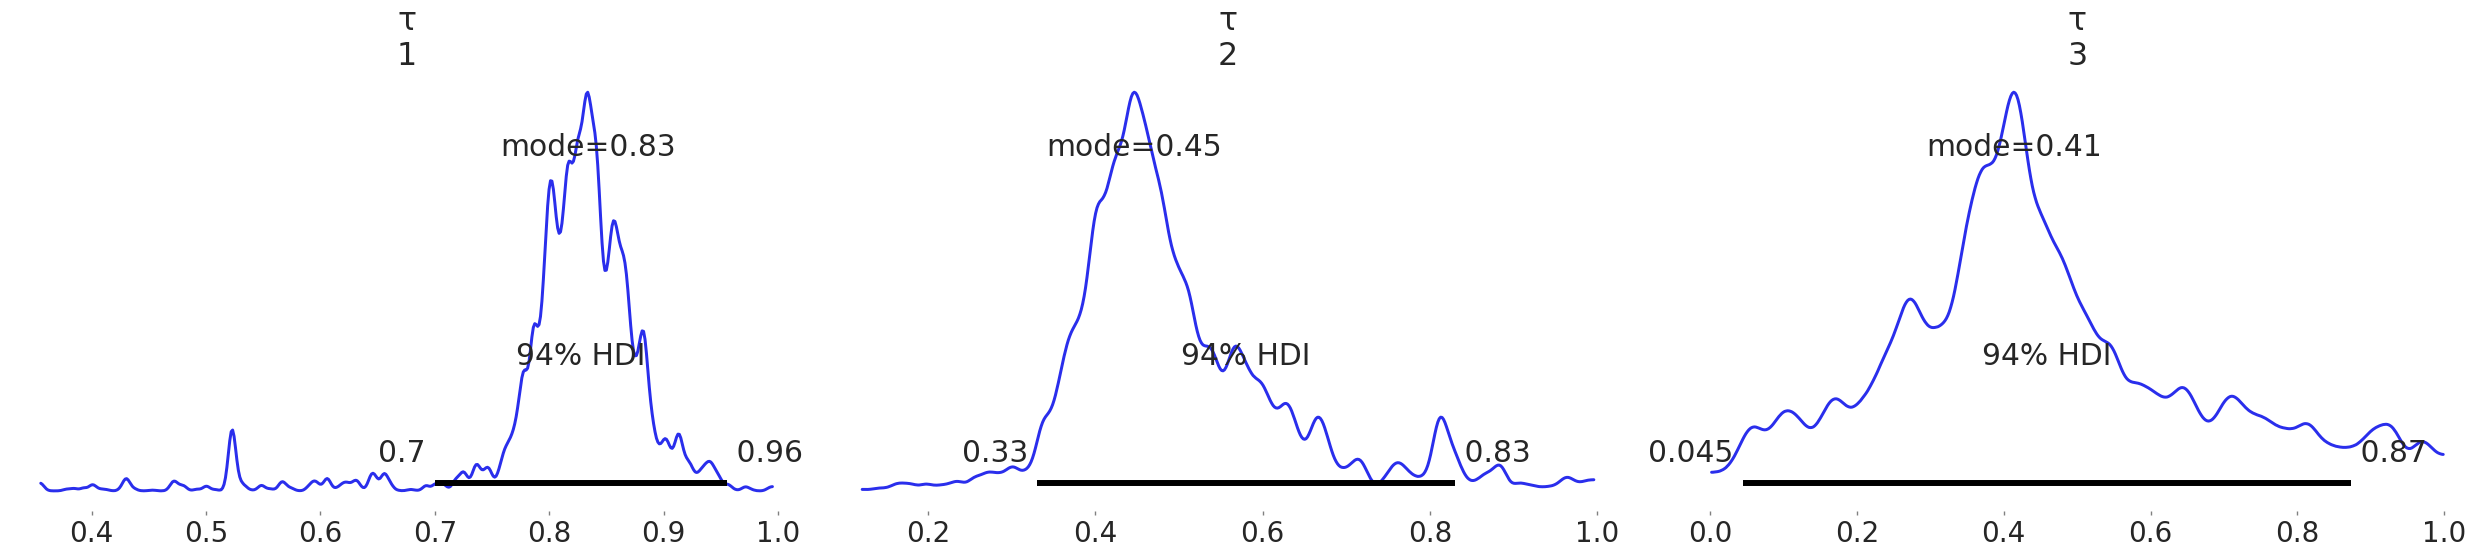
\includegraphics[width=.9\textwidth]{credible_intervals}}
  \caption{Example of 94\% credible intervals on the posterior distribution of the impact points}\label{fig:credible_intervals}
\end{figure}


Moreover, we can perform various visual checks, such as a plot comparing both the observed and posterior predictive distribution of the responses (see Figure~\ref{fig:ppc}). The posterior predictive distribution for a new sample \(x\) is formally defined as
\[
\pi(y\mid x, \mathcal D_n) = \int_{\Theta} \pi(y\mid x, \theta)\pi(\theta\mid \mathcal D_n)\, d\theta,
\]
and in our context it can be approximated by the simulated responses \(\symbf Y^* \equiv \{\symbf Y^{(m)*}\}\), following the notation of~\eqref{eq:sampled-response-vector}. This distribution accounts for the uncertainty about \(\theta\), and we do indeed use it for prediction in our predict-then-summarize approach.

\begin{figure}[ht!]
  \centering
  \setlength{\fboxrule}{.5pt}%
  \fbox{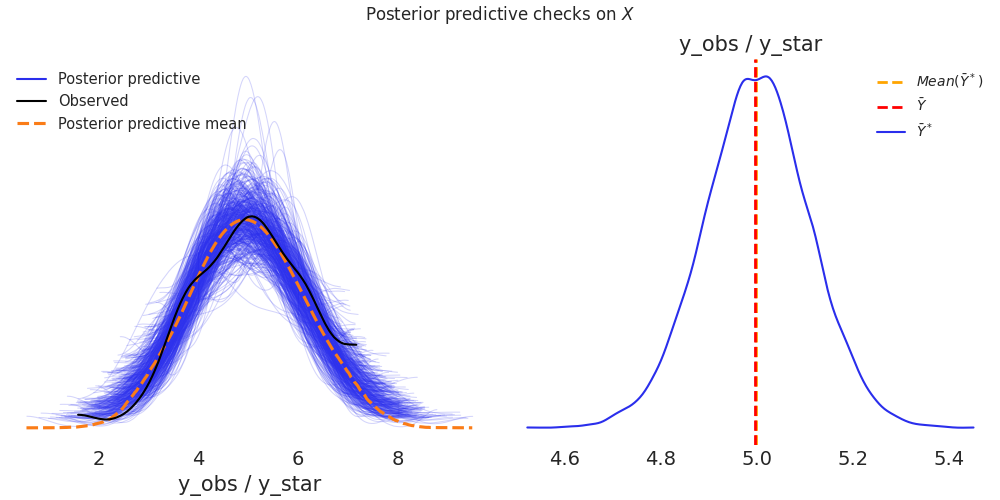
\includegraphics[width=.65\textwidth]{ppc_linear}}
  \caption{Example of posterior predictive graphical checks on a fitted linear regression model. We show a comparison between the observed distribution of the response variable and the posterior predictive distribution consisting on the approximate sampled responses.}\label{fig:ppc}
\end{figure}


In addition, we can calculate the so-called \textit{Bayesian p-values} for several statistics, which are defined as \(P(T(\symbf Y^*)\leq T(\symbf Y)| \symbf Y)\), and are computed by simply measuring the proportion of the \(M\) estimates \(T\{\symbf Y^{(m)*}\}\) that fall below the observed value of the statistic, \(T(\symbf{Y})\). They are expected to be around 0.5 when the model accurately represents the data, and a deviation either way can be indicative of modeling issues; see Chapter 6 of \citet{gelman2013bayesian} for details.
